% Class diagram of the order management domain (workshop step 1).
% Standalone file: compile with  pdflatex class-diagram.tex
% To reuse it in the report, copy the tikzpicture environment into your document
% (preamble needs: \usepackage{tikz} and the libraries listed below).
\documentclass[tikz,border=8pt]{standalone}
\usetikzlibrary{positioning,arrows.meta,shapes.multipart,calc}

\begin{document}
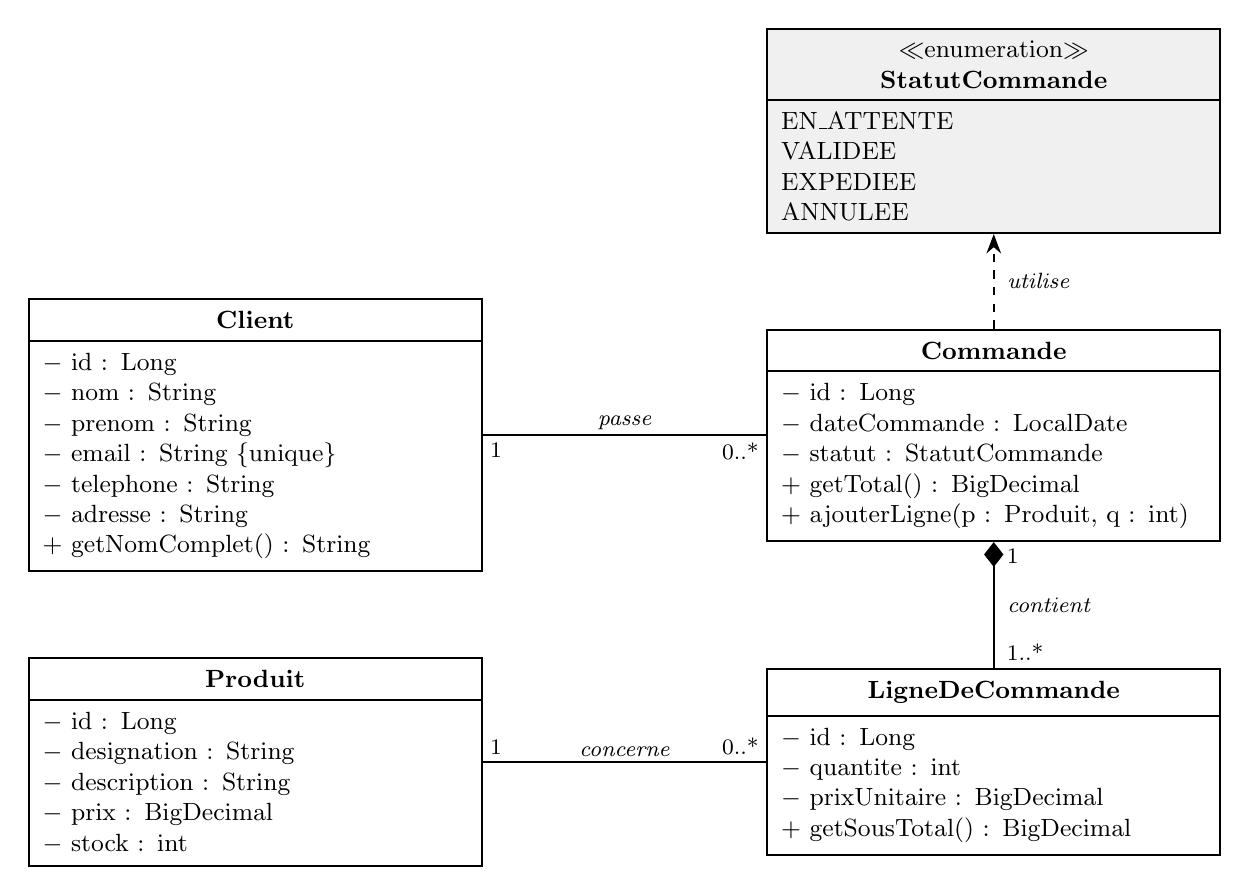
\begin{tikzpicture}[
    font=\small,
    node distance=1.6cm and 3.6cm,
    class/.style={rectangle split, rectangle split parts=2, draw, thick, fill=white,
                  text width=5.4cm, inner xsep=5pt, inner ysep=4pt, align=left},
    enum/.style={rectangle split, rectangle split parts=2, draw, thick, fill=black!6,
                 text width=5.4cm, inner xsep=5pt, inner ysep=4pt, align=left},
    assoc/.style={thick},
    mult/.style={font=\footnotesize, inner sep=1.5pt},
    role/.style={font=\footnotesize\itshape, fill=white, inner sep=1.5pt}
]

% ---------------------------------------------------------------- classes

\node[class] (commande) {
    \centerline{\textbf{Commande}}
    \nodepart{second}
    $-$ id : Long \\
    $-$ dateCommande : LocalDate \\
    $-$ statut : StatutCommande \\
    $+$ getTotal() : BigDecimal \\
    $+$ ajouterLigne(p : Produit, q : int)
};

\node[class, left=of commande] (client) {
    \centerline{\textbf{Client}}
    \nodepart{second}
    $-$ id : Long \\
    $-$ nom : String \\
    $-$ prenom : String \\
    $-$ email : String \{unique\} \\
    $-$ telephone : String \\
    $-$ adresse : String \\
    $+$ getNomComplet() : String
};


\node[class, below=of commande] (ligne) {
    \centerline{\textbf{LigneDeCommande}}
    \nodepart{second}
    $-$ id : Long \\
    $-$ quantite : int \\
    $-$ prixUnitaire : BigDecimal \\
    $+$ getSousTotal() : BigDecimal
};

\node[class, left=of ligne] (produit) {
    \centerline{\textbf{Produit}}
    \nodepart{second}
    $-$ id : Long \\
    $-$ designation : String \\
    $-$ description : String \\
    $-$ prix : BigDecimal \\
    $-$ stock : int
};

\node[enum, above=1.2cm of commande] (statut) {
    \centerline{$\ll$enumeration$\gg$}
    \centerline{\textbf{StatutCommande}}
    \nodepart{second}
    EN\_ATTENTE \\ VALIDEE \\ EXPEDIEE \\ ANNULEE
};

% ---------------------------------------------------------------- relations
% Client 1 --- 0..* Commande
\draw[assoc] (client.east) -- node[role, above] {passe} (commande.west);
\node[mult, below right=1pt and 1pt] at (client.east)   {1};
\node[mult, below left=1pt and 1pt]  at (commande.west) {0..*};

% Commande <>--- 1..* LigneDeCommande (composition)
\draw[assoc, {Diamond[length=9pt,width=7pt,open=false,fill=black]}-] (commande.south) --
    node[role, right=3pt] {contient} (ligne.north);
\node[mult, below right=1pt and 3pt] at (commande.south) {1};
\node[mult, above right=1pt and 3pt] at (ligne.north)    {1..*};

% LigneDeCommande 0..* --- 1 Produit
\draw[assoc] (ligne.west) -- node[role, above] {concerne} (produit.east);
\node[mult, above left=1pt and 1pt]  at (ligne.west)   {0..*};
\node[mult, above right=1pt and 1pt] at (produit.east) {1};

% Commande uses StatutCommande (dependency)
\draw[-{Stealth[length=7pt]}, dashed, thick] (commande.north) -- node[role, right=3pt] {utilise} (statut.south);

\end{tikzpicture}
\end{document}
